%%%%%%%%%%%%%%%%%%%%%%%%%%%%%%%%%%%%%%%%%%%%%%%%%%%%%%%%%%%%%%%%%%%%
%% chapter3.tex
%% UNL thesis document file
%%
%% Chapter with a short laext tutorial and examples
%%%%%%%%%%%%%%%%%%%%%%%%%%%%%%%%%%%%%%%%%%%%%%%%%%%%%%%%%%%%%%%%%%%%
\chapter{State Of the Art}
\label{cha:stateofart}

\acresetall

In the previous chapter the complexity and multimodality of communication was presented by explaining the anatomical actors involved. It was also shown how easily speech production can be affected through neurological diseases. To study communication, especially impaired communication caused by motoric speech disorders, this chapter outlines the state-of-the-art from different areas which can be used to study communication from a computational perspective. 

Given the multimodality of communication, this chapter starts with an overview of non-invasive sensors able to detect facial activity as well as blood flow and other communication properties. As emotion expression can affect speech, its detection diverse modalities will be elaborated in this chapter, especially as it has been shown to provide indicators to detect mental disorders and showed that \gls{pdg} and \gls{adg} patients have reduced facial expressions. 

In chapter~\ref{sec:afer} a special focus is put on \gls{aferg} by presenting its taxonomy and algorithms used as motoric speech disorders can affect not only muscles needed for speech production, but also those needed to express emotions. Also remaining challenges in \gls{afer} will be listed.

This chapter ends with an overview of multimodal machine learning (MML) and its challenges.A deeper insight is given in the representation of multimodal data and data fusion.


\section{Computational Communication Analysis }
\label{sec:compcommunication}

As communication is a multimodal activity, different modalities are necessary to analyze communication from a computational perspective. In Table~\ref{tab:modality} several modalities which can be used to collect data and analyze communication properties are listed. Audio data permits the analysis of speech sounds, voice prosody and other paralinguistic characteristics, as well as speech recognition which is focused on understanding the meaning of what is said. RGB data is used to detect \gls{aug} and underlying emotions. Important for non-verbal communication is oculesics analysis (e.g., pupil dilation and eye movements) which can be indicators of attention and arousal. Thermal imaging can provide information of airflow and blood flow. The latter can be used as indicator of emotions such as momentary stress (increased the periorbital blood flow) and joy (decreased blood flow to the nose)\cite{Corneanu2016survey}. Depth information is specially useful when the face cannot be recorded frontally to detect facial expressions. \gls{eeg} can also be used to measure arousal and valence of certain emotions. \gls{eda} measures skin conductance (sweat) which has been shown to be an indicator for stress, anxiety, and has been used as well for clinical assessment of pain and schizophrenia \cite{Chen2015wavelet}.


\begin{table}
\centering
\caption{Overview of different modalities and what communication properties they analyze.}
\label{tab:modality}
\begin{tabular}{l|l}
\toprule
\textbf{Modality}      & \textbf{Communication properties}                 \\ \midrule
\multirow{2}{*}{Audio} & voice analysis (study of speech sounds)           \\
                       & speech recognition (study of linguistic contents) \\ \midrule
\multirow{3}{*}{RGB}   & facial expression detection                       \\
                       & gaze analysis                                     \\
                       & pupil dilation                                    \\ \midrule
Thermal                & airflow                                           \\
                       & blood flow                                        \\ \midrule
Depth                  & facial expression detection                       \\ \midrule
\multirow{2}{*}{EEG}   & arousal                                           \\
                       & valence                                           \\ \midrule
EDA                    & skin conductance                                 
\end{tabular}
\end{table}


%--------------------------------------------------------
\subsection{Facial Expression detection in Health disorders}

Computational face detection and recognition is part of the field computer vision and had its beginnings in the 1960's \cite{Bledsoe1966}. From there on several algorithms were developed \cite{Zhao2003}, including the Viola \& Jones algorithm in 2001 which is still state-of-the art \cite{Viola2001}. However, with the
introduction of the term "Affective Computing" in 1995 by Rosalind Picard a new line of research emerged, namely \gls{aferg} which is the recognition of \glspl{fe} giving insights about the emotional state of a person \cite{Huang2010,Anil2016,Pantic2000,Sariyanidi2015}. Based on the contribution done in \cite{Ekman1977} it became possible to categorize facial muscle contractions and label data using the created taxonomy \gls{facs} (see Fig.~\ref{fig:facs}). In \cite{Ekman1997} the different facial contractions also called \glspl{au} were combined and related to emotions permitting the research of computational affect recognition.

The detection of emotions has several applications but recently it gained more and more interest in the research community for use in \gls{behaviomedics}\cite{Valstar2014automatic}. The analysis of emotions using video data has been used to detect mental disorders, such as stress, anxiety, and depression \cite{Holt2016,Valstar2014automatic,Valstar2016avec,Valstar2014avec}. 

Face analysis has also been applied to diagnose eating disorders \cite{Leppanen2017} and estimate pain intensity \cite{Valstar2014automatic}, using, for instance, recurrent \glspl{cnn} \cite{Zhou2016}. 

Also neurodegenerative diseases such as \gls{pd} \cite{Almutiry2016,Bandini2017,Silverdale2016} and \gls{ad} have been studied using facial expression analysis. Deficits in the mimicry of facial expressions were detected by \cite{Livingstone2016} and \cite{Ricciardi2015} confirmed reduced facial expressions. In \cite{Cadieux1997} 
emotion processing in \gls{ad} was studied and in \cite{Gola2017} it was shown that patients suffer deficits in the ability to intentionally imitate \glspl{fe} of emotion.

Also autism has been studied by classifying \gls{fe} based on video data \cite{Valstar2014automatic} as this disorder causes difficulty in reading faces and show deficits in non-verbal as well as in verbal communication.

%-------------------------------------------------
\subsection{Audio Analysis for Speech Disorders and Emotion Detection}

Also in speech analysis the interest in detecting emotions grew. In \cite{Anagnostopoulos2015survey} the history from 2000-2011 of the different features and classifiers used for emotion recognition from speech is presented. However, as happened with emotion detection through video analysis, the interest changed to detection and severity deduction of diseases. In \cite{Cummins2016} and \cite{Singh2017} mental diseases are detected and graded in severity using paralinguistic analysis. Also speech of Alzheimer's disease patients have been studied \cite{Lopez-de-Ipina2015b,Lopez-de-Ipina2014} to detect the 
impairment of vocal expression of negative emotions\cite{Zaytseva2014,Lopez-de-Ipina2015} and general impairment of emotional prosody \cite{Horley2010}. In  \cite{Schuller2015interspeech,Moebes2008,Zhao2014} speech of patients with Parkinson's Disease have been studied and it was shown that alterations of emotional processing contribute to speech changes in Parkinson's Disease, especially regarding emotional prosody, in addition to motor impairment.

Also speech stuttering has been analyzed through audio. \cite{Hariharan2012} used sample entropy and Least Square Support Vector Machine to assess speech stuttering. To detect dysfluency (stuttering) \cite{jhawar2016speech} used mel frequency cepstral coefficients (MFCC) and \cite{Ramteke2016} additionally dynamic time warping (DTW). For prolongation recognition \cite{Chee2009} used MFCC and \cite{Savin2016} ANNs. To classify different stuttering types \cite{Mahesha2016} used Gaussian mixture models (GMM), \cite{Mahesha2015} used SVMs, and \cite{Pravin2017} ANNs.



\begin{comment}
-	What are the state-of-the-art techniques?\\
-	What are the challenges to detect speech disorders?\\

\subsection{Datasets}
new generation of databases: \cite{DouglasCowie2003}\\



\url{http://vkc.mc.vanderbilt.edu/childhoodstuttering/forscientists_datasets.html}\\

paper: The UCLASS archive of stuttered speech\\
\end{comment}



%-------------------------------------------------
\subsection{Physiological Signals for Emotion Detection}

The modalities presented before, show that it is possible to detect affect, which is the expression of emotions which can be observed. However, research has wondered if it possible to detect the emotion itself using physiological data. Nevertheless, whether EEG, e.g., just shows a physiological response, or also gives insight into the emotion as how it is experienced mentally, is still unclear. Some of those most commonly used physiological signals have been: electrocardiogram (ECG) and related heart rate variability series, \gls{eda}, respiration, muscle activity, peripheral temperature, eye gaze, as well as brain activity (\gls{eeg}) \cite{Wang2014}.


Among these, EDA has been widely used to assess the arousal level in humans because of its
ability to quantify changes in the sympathetic nervous system (SNS).
In \cite{Walkom2016virtual} \gls{eda} was used to measure anxiety levels in \gls{pws} while they presented a talk to a virtual audience. This Virtual Reality Exposure Therapy (VRET) showed improvements in speech for the participants of this study as it helped the participants handle social anxiety. Also in \cite{Shamsi2016} a relation between stress measured with \gls{eda} and stuttering could be shown. However, it was not precised whether the stuttering began through increased stress or whether the stuttering caused the stress increasing.

In \cite{Soleymani2016analysis} data was collected with EEG and video to detect emotions of a video's viewer. They found the results from facial expressions to be superior to the results from EEG signals. They analyzed the effect of the contamination of facial muscle activities on EEG signals and found that most of the emotionally valuable content in EEG features are as a result of this contamination. However, the statistical analysis showed that EEG signals still carry complementary information in presence of facial expressions.

In \cite{Bocharov2017depression} EEG was used to evaluate the difference between low depression (LD) and high depression (HD). The findings were that HD scorers evidence increased emotional arousal to negative and decreased emotional arousal to positive stimuli during implicit emotion processing. 

% ==================================================================
\section{Automated Facial Expression Recognition (AFER)}
\label{sec:afer}

\begin{figure}
    \centering
    
\includegraphics[width=14cm]{FEdetectiondiagram}
    \caption{Steps necessary for \gls{afer}.}
    \label{fig:FEdiagram}
\end{figure}

\gls{afer} is composed of four main steps shown in Fig.~\ref{fig:FEdiagram}\cite{Cohn2014,Fasel2003}. Face localization is necessary to separate the human face from the background, using e.g., the Viola \& Jones algorithm. Face registration, also known as alignment for 2D cases, is necessary to rotate or frontalize the face. For this step specific stable landmarks such as eye corners and nose can be used. For further processing features are extracted which can be predesigned or learned (see Fig.~\ref{fig:AFER}). Learned features are automatically learned from data using for instance deep learning techniques \cite{Jaiswal2016}, which jointly learn the feature extraction and classification or regression weights. These categories are further divided into global and local, where global features extract information from the whole facial region, and local ones from specific regions of interest, usually corresponding to \glspl{au}. Features can also be split into static and dynamic, with static features describing a single frame or
image and dynamic features being image sequences\cite{Valstar2006}. Predesigned features can be divided into appearance and geometrical\cite{Mishra2015}. The former use the intensity information of the image \cite{Lucey2007}, while the latter measure distances, deformations, curvatures and other geometric properties. This is not the case for learned features, as the nature of the extracted information is usually unknown.

\Gls{fe} classification can be grouped into categorical and continuous depending on the target expressions\cite{Tian2005}. For categorical classification, a set of expressions is predefined\cite{Chu2016}. Commonly a classifier is trained for each one, using e.g. \glspl{svm}\cite{Simon2010}, on the six primary expressions - happiness, sadness, surprise, fear, disgust, and anger. In continuous classification \glspl{fe} are represented as points in a
continuous multidimensional space \cite{Zeng2009survey}. This permits the representation of subtly different
expressions, mixtures of primary expressions, and to define them through clustering in an unsupervised manner. 

An overview of available datasets for \gls{fe} recognition can be viewed in Table~\ref{tab:rgbDatasets}.


\begin{figure}
{\footnotesize
\begin{forest}
    for tree={
      edge path={
        \noexpand\path [draw, thick, \forestoption{edge}] (!u.parent anchor) -- +(5pt,0) |- (.child anchor)\forestoption{edge label};
      },
      parent anchor=east,
      child anchor=west,
      grow'=east,
      text centered,
      minimum width=1in,
      text width=2.4cm
      }
 [Automatic\\  Facial\\ Expression Recognition [Parametrization [Descriptive] [Judgement]] [Recognition [Face \\ localization [Detection] [Segmentation]] [Face \\ registration] [Feature \\ extraction [Predesigned [Appearance][Geometry][Appearance + Geometry]][Learned]] [Expression\\ Classification /Regression [Categorical] [Continuous]] [Multimodal \\fusion [Direct fusion][Early fusion][Late fusion] [Sequential]]]]
  \end{forest}
}
\caption{Taxonomy for AFER adapted from \cite{Corneanu2016survey}.}
\label{fig:AFER}
\end{figure}



%------------------------------------------
\subsection{Techniques used in 3D and Thermal imaging for AFER}

With the advancement of camera sensor technology alternative modalities to RGB have been used in research for \gls{afer}, such as 3D and thermal cameras. In the following, strengths and weaknesses of those modalities will be described \cite{Corneanu2016survey}.

\paragraph{3D}
Face localization in 3D images can be done using curvature features to detect high curvature areas such as the nose tip and eye cavities\cite{Colombo2006}. Segmentation can also be applied in order to remove the background by detecting edges and ellipsoids and applying k-means to select the highest probability fitting \cite{Segundo2010}.
Face registration is then performed by minimizing the distance between the acquired geometry and a shape model. Iterative closest point (ICP) \cite{Besl1992} iteratively aligns
the closest points of two shapes. In \cite{Alyuz2012}, visible patches of
the face are detected and used to discard obstructions before using ICP for alignment. In the case of non-rigid registration,
it allows the matched 3D model to deform. 


Geometric features in 3D are similar to those in RGB data as the distance between pairs of 3D
landmarks are used \cite{Tang2008}. Manifolds such as Lipschitz embeddings can be used to describe the shape deformation of a fitted 3D mesh separately at each frame of a video sequence \cite{Chang2005automatic}. On the contrary to RGB and 3D data, however, appearance features cannot be used as 3D data does not convey appearance information.



\paragraph{Thermal}

In thermal images, RGB techniques can be applied for face localization, however, segmenting the image according to the radiant emittance of each pixel usually is enough \cite{Koda2009facial}.
Nevertheless, methods for feature extraction used in RGB data, such as geometric features,  cannot be extracted from thermal data, since
dull facial features difficult the precise localization of landmarks. Therefore global appearance features are used based on standard feature descriptors such as Gabor filters\cite{Littlewort2011}, pyramids
of histograms of gradients\cite{Dhall2011emotion}, multi-scale dense SIFT\cite{Sun2014combining}, and LBP\cite{Shan2009facial}, to exploit the difference of temperature between
regions.



An overview of available datasets for 3D, and thermal data can be seen in Table~\ref{tab:3DThermaldatasets}.


\begin{sidewaystable}
\centering
\caption{Non-comprehensive list of RGB datasets for \gls{fe} recognition adapted from \cite{Corneanu2016survey}.}
\label{tab:rgbDatasets}
\resizebox{!}{.2\paperwidth}{%
\begin{tabular}{l p{3cm} ccccccccccc}
\toprule
                          &                                         & \multicolumn{11}{c}{\textbf{RGB}}                                                                      \\ \cmidrule{3-13}
                          &                                         & \textbf{CK+}   & \textbf{MPIE}     & \textbf{JAFFE} & \textbf{MMI}   & \textbf{RU\_FACS} & \textbf{SEMAINE} & \textbf{CASME}  & \textbf{DISFA} & \textbf{AFEW}  & \textbf{SFEW} & \textbf{AMFED} \\ \midrule
\multirow{2}{*}{\textbf{Content}}                   & Intention \footnotesize{(\textbf{P}osed/\textbf{S}pontaneous)}   & P     & P        & P     & P     & S        & S       & S      & S     & S     & S    & S     \\
                   & Temporality \footnotesize{(\textbf{S}tatic/\textbf{D}ynamic)}    & D     & S        & S     & D     & D        & D       & D      & D     & D     & S    & D     \\ \midrule
\multirow{4}{*}{\textbf{Capture}}  & Environment \footnotesize{(\textbf{L}ab/in the \textbf{W}ild)} & L     & L        & L     & L     & L        & L       & L      & L     & N     & N    & N     \\
                          & \parbox[t]{3cm}{Multiple\\ Perspective}                    & no    & yes      & no    & yes   & yes      & no      & no     & no    & yes   & yes  & yes   \\
                          & \parbox[t]{3cm}{Multiple\\ Illumination}                   & no    & yes      & no    & yes   & no       & no      & no     & no    & yes   & yes  & yes   \\
                          & Occlusions                              & no    & yes      & no    & no    & yes      & no      & no     & no    & yes   & yes  & yes   \\ \midrule
\multirow{4}{*}{\textbf{Subjects}} & \# of subjects                          & 201   & 337      & 10    & 75    & 100      & 150     & 35     & 27    & 220   & 68   & 5268  \\
                          & Ethnic Diverse                          & yes   & yes      & no    & yes   & no       & no      & no     & yes   & yes   & yes  &       \\
                          & Gender \footnotesize{(M/F(\%))}               & 31/69 & 70/30    & 100/0 & 50/50 & -        & 62/38   & 37/63  & 44/56 & -     & -    & 58/42 \\
                          & Age                                     & 18-50 & $\mu=27.9$ & -     & 19-62 & 18-30    & 22-60   & $\mu=22$ & 18-50 & 18-70 & -    & -     
\end{tabular}}
\end{sidewaystable}



\begin{sidewaystable}[]
\centering
\caption{Non-comprehensive list of 3D and thermal datasets for \gls{fe} recognition adapted from \cite{Corneanu2016survey}.}
\label{tab:3DThermaldatasets}
\begin{tabular}{llcccccccc}
\toprule
                          &                                         & \multicolumn{4}{c}{\textbf{3D}}                & \multicolumn{4}{l}{\textbf{RGB+Thermal}} \\ \cmidrule(l){3-6}\cmidrule(l){7-10} 
                          &                                         & \textbf{BU-3DFE} & \textbf{BU-4DFE} & \textbf{Bosphorus} & \textbf{BP4D}  & \textbf{IRIS}  & \textbf{NIST}  & \textbf{NVIE}   & \textbf{KTFE}   \\ \midrule
\multirow{2}{*}{\textbf{Content}}  & Intention \footnotesize{(\textbf{P}osed/\textbf{S}pontaneous)}   & P       & P       & P         & S     & P     & P     & S/P    & S/P    \\
                          & Temporality \footnotesize{(\textbf{S}tatic/\textbf{D}ynamic)}    & S       & D       & S         & D     & S     & S     & D      & D      \\ \midrule
\multirow{4}{*}{\textbf{Capture}}  & Environment \footnotesize{(\textbf{L}ab/in the \textbf{W}ild)} & L       & L       & L         & L     & L     & L     & L      & L      \\
                          & Multiple Perspective                    & yes     & yes     & -         & yes   & yes   & yes   & yes    & yes    \\
                          & Multiple Illumination                   & no      & no      & no        & no    & yes   & yes   & yes    & yes    \\
                          & Occlusions                              & yes     & no      & yes       & no    & yes   & yes   & yes    & yes    \\ \midrule
\multirow{4}{*}{\textbf{Subjects}} & \# of subjects                          & 100     & 101     & 105       & 41    & 30    & 90    & 215    & 26     \\
                          & Ethnic Diverse                          & yes     & yes     & no        & yes   & yes   & -     & no     & no     \\
                          & Gender \footnotesize{(M/F(\%))}              & 56/44   & 57/43   & 43/57     & 56/44 & -     & -     & 27/73  & 38/62  \\
                          & Age                                     & 18-70   & 18-45   & 25-35     & 18-29 & -     & -     & 17-31  & 12-32 
\end{tabular}
\end{sidewaystable}





%--------------------------------------------------------

\subsection{Challenges in AFER}

In \gls{afer}, two main long-term challenges can be defined: 1) in-the-wild \gls{afer}, and 2) inclusion of \gls{afer} in a multimodal framework modelling human behavior.\cite{Martinez2016}

1) Currently \gls{afer} is tested on high quality data recorded under controlled lab conditions, displaying subjects frontally with frontal illumination and no self occlusions.Also expressive behavior is often elicited under controlled conditions, using video clip stimuli or involving human-computer interaction tasks.
These conditions reduce the complexity of the data, which otherwise is found in natural environments.

2) Human behavior as well as communication is currently analyzed from different perspectives, whereby facial expressive behavior is only one component. In order to understand humans, a multimodal framework in which different information from audio, \glspl{fe}, and head-pose for instance, are analyzed jointly, rather than separately to obtain a big picture.  

Besides the long-term challenges, the following problems need to be tackled \cite{Martinez2016}:
\begin{enumerate}
\item Data
\item Semi-automatic annotation
\item Label subjectivity
\item Avoiding dataset biases
\item Finding a better representation
\item Occlusions
\item Dynamics
\item From momentary to higher-level
\item Computational efficiency
\end{enumerate}




Although \gls{afer} has grown rapidly in recent years most evaluations still focus on either posed expressions, near-frontal
recordings, or both. To test how existing recognition approaches perform in conditions with a wide range of poses the 
Facial Expression Recognition and Analysis challenge (FERA 2017) provided data to estimation the occurrence and intensity of \glspl{au} under different camera views. 





\begin{comment}
challenges: face pose FERA2017 \cite{Valstar2017}

 advances, challenges and opportunities \cite{Martinez2016}

To compare methods on the same dataset, the AVEC challenge was created. \cite{Valstar2016avec}\cite{Valstar2014avec}

occluded faces \cite{Cotter2010}, automated face and gesture recognition \cite{de2015intraface}, advances, challenges and opportunities \cite{Martinez2016}\\


 3D \cite{Danelakis2015}survey\cite{Sandbach2012survey}




3d motion analysis of facial movement during verbal and nonverbal expressions in healthy subjects \cite{Sidequersky2016}\\

comparison 2d vs 3d automatic FACS detection \cite{Savran2012}\\
\end{comment}
% ===============================================================

% ===============================================================
\begin{comment}
\section{Physiological Data Analysis in Speech Disorders and Emotion Analysis}

EEG:\\
-	Has it been used to analyze stuttering, apraxia or dysarthria?\\
-	Has it been used for emotion detection?\\
-	Used to measure concentration?\\
-	What are the state-of-the-art techniques?\\
-	What are the challenges?\\

classification of stuttering and non-stutterer \cite{saltuklaroglu2017eeg}

classification of stuttering types: using brain activity\cite{Jiang2012}

EDA:\\
-	How has it been used for emotion detection?\\
-	What are the applications/studies about?\\
-	Has it been used for speech disorders?\\
-	Has it been used as biofeedback to improve speech?\\
-	What are the state-of-the-art techniques?\\
-	What are the challenges?\\

\end{comment}

% ===============================================================

\section{Multimodal Machine Learning}
\label{sec:multiML}
\begin{comment}
Audiovisual emotion recognition \cite{Chao2016}, \cite{Corneanu2016survey}, \cite{Nicolle2012}, survey \cite{Zeng2009survey}\\

face analysis for speech detection (lip-reading, audio-visual speech):\\

A review of affective computing: From unimodal analysis to multimodal fusion\cite{Poria2017}\\

 eating condition audio-visual\cite{Schuller2015interspeech}

multimodal audio-video and physiological data AVEC2015 \cite{Ringeval2015}\\
\end{comment}


Information is being exchanged through different channels. These different channels can be called modalities. The same way humans can process information coming from different sources in order to take conclusions and take action, the ultimate goal of artificial intelligence is to understand the world around us by collecting, interpreting and reasoning multimodal data. This field can be called \textbf{Multimodal Machine Learning} which aims to build models that can process and relate information from multiple modalities and which is gaining more and more importance and has extraordinary potential \cite{Baltruvsaitis2017multimodal}.

Although Multimodal Machine Learning brings many challenges given the heterogeneity of data, the hope is to gain a deeper understanding of natural phenomena as data from multimodal sources are used to capture correspondences between the modalities.

One of the first examples of multimodal research is audio-visual speech recognition (AVSR) in 1989. The motivation came from the discovered McGurk effect in which it was found that human perception of sound is not independent from the visual perception. During the experiment subjects heard the syllable /ba-ba/ while they the lips of a person saying /ga-ga/, however, they perceived the sound /da-da/. Researcher from the speech community started to include visual information in their investigations. Although research in AVSR is not common currently, the deep learning community showed renewed interest \cite{Ngiam2011}. What was shown in the experimental results in AVSR is that the captured interactions between speech and visual information were not complementary but rather supplementary. Experimental results showed more advantage of using visual information when the speech signal was noisy but not when the scenario was noiseless.
In \cite{Dmello2015review} several multimodal affect recognition results were compared and their meta-analysis revealed that a majority of recent work on multimodal affect recognition showed an improvement when using more than one modality. However, the improvement on naturally-occurring emotions is reduced. 

There are main challenges (taken from \cite{Baltruvsaitis2017multimodal}, \todo{rephrase}):
\begin{enumerate}
\item \textbf{Representation:} A first fundamental challenge is learning how to represent and summarize multimodal data in a way that exploits the complementarity and redundancy of multiple modalities. The heterogeneity of multimodal data makes it challenging to construct such representations. For example, language is often symbolic while audio and visual modalities will be represented as signals.
\item \textbf{Translation:} A second challenge addresses how to translate (map) data from one modality to another. Not only is the data heterogeneous, but the relationship between modalities is often open-ended or subjective. For example, there exist a number of correct ways to describe an image and and one perfect translation may not exist.
\item \textbf{Alignment:} A third challenge is to identify the direct relations between (sub)elements from two or more different modalities. For example, we may want to align the steps in a recipe to a video showing the dish being made. To tackle this challenge we need to measure similarity between different modalities and deal with possible longrange dependencies and ambiguities.
\item \textbf{Fusion:} A fourth challenge is to join information from two or more modalities to perform a prediction. For example, for audio-visual speech recognition, the visual description of the lip motion is fused with the speech signal to predict spoken words. The information coming
from different modalities may have varying predictive power and noise topology, with possibly missing data in at least one of the modalities.
\item \textbf{Co-learning:} A fifth challenge is to transfer knowledge between modalities, their representation, and their predictive models. This is exemplified by algorithms of cotraining,
conceptual grounding, and zero shot learning.
Co-learning explores how knowledge learning from one modality can help a computational model trained on a different modality. This challenge is particularly relevant when one of the modalities has limited resources (e.g., annotated data).
\end{enumerate}

%---------------------------------
\subsection{Multimodal Representations}
\label{sec:multiRepr}
\todo{rephrase}
Following the work of \cite{Bengio2013representation} the term feature and representation are used interchangeably, with each referring to a vector or tensor representation of an entity, be it an image, audio sample, individual word, or a sentence. A multimodal representation is a representation of data using information from multiple such entities. Furthermore, the representation of the data is the backbone of any multimodal model. Good representations are important for the performance of machine learning models.

However, there are different challenges when it comes to represent multimodal data: how to combine data from heterogeneous sources; how to deal with different levels of noise; and how to deal with missing data.  \cite{Baltruvsaitis2017multimodal}

In \cite{Bengio2013representation} the following characteristics of good representations are listed: smoothness, temporal and spatial coherence, sparsity, and natural clustering amongst others. In \cite{Srivastava2012} additional desirable properties for multimodal representations are listed, e.g., the similarity in the representation space should reflect similarity of the corresponding concepts, the representation should be easy to obtain even in the absence of some modalities, and it should be possible to fill-in missing modalities given observed ones.

Unimodal representations have been studied extensively in the past and recently a shift has been observed from hand-designed representations (e.g. SIFT) for specific applications to data-driven using f.ex. \glspl{cnn}. Until recently multimodal representations involved simple concatenation of unimodal ones but this has been changing rapidly.

According to \cite{Baltruvsaitis2017multimodal} there are two types of multimodal representation: joint and coordinated. 

\paragraph{Joint representations} combine unimodal signals into the same representation space:$x_m = f(x_1, \cdots, x_n)$.
The multimodal representation $x_m$ is computed using function $f$ through, e.g., a deep neural network, restricted Boltzmann machine, or a recurrent neural network that relies on unimodal representations $x_1,\cdots, x_n $. 
Joint representations are mostly used in tasks where multimodal data is present during training and inference steps. One example is early fusion which is the simple concatenation of individual modality features. More advanced methods are \textit{neural networks}, \textit{graphical models} and \textit{recurrent neural networks}.

\underline{\textit{Neural networks}} are very popular for unimodal representation such as visual, acoustic, and textual data, and are increasingly used in the multimodal domain.
In general, neural networks are made up of successive building blocks of inner products followed by non-linear activation functions. In order to use a neural network as a way to represent data, it is first trained to perform a specific task (e.g., recognizing objects in images). Due to the multilayer nature of deep neural networks each successive layer is hypothesized to represent the data in a more abstract way \cite{Bengio2013representation}, hence it is common to use the final or penultimate neural layers as a form of data representation. To construct a multimodal representation using neural networks each modality starts with several individual neural layers followed by a hidden layer that projects the modalities into a joint space \cite{Mroueh2015deep}. The joint multimodal representation is then passed through multiple hidden layers itself or used directly for prediction. Such models can be trained end-to-end — learning both to represent the data and to perform a particular task.
This results in a close relationship between multimodal representation learning and multimodal fusion when using neural networks.
The major advantage of neural network based joint representations comes from their often superior performance and the ability to pre-train the representations in an unsupervised
manner. The performance gain is, however, dependent on the amount of data available for training. One of the disadvantages comes from the model not being able to handle missing data naturally — although there are ways to alleviate this issue \cite{Ngiam2011}. Finally, deep networks are often difficult to train \cite{Glorot2010understanding}, but the field is making progress in better training techniques

\underline{\textit{Probabilistic graphical models}} construct representations using latent random variables. Popular approaches are deep Boltzmann machines (DBM) which stack restricted Boltzmann machines (RBM) as building blocks. Similar to neural networks, each layer represents the data at a higher level of abstraction. The advantage is that DBM do not need supervised data for training. These graphical models represent the data in a probabilistic manner, but it can be converted to deterministic neural networks with the cost of loosing the generative aspect of the model which allows to deal with missing data even if a whole modality is missing.
Multimodal deep belief networks have been extended to multimodal DBMs which are able to learn joint representations from multiple modalities by merging two or more undirected graphs using a binary layer of hidden units on top of them. They allow for the low level representations of each modality to influence each other after the joint training due to the undirected nature of the model. Similar to autoencoders the representation can be trained in an unsupervised manner enabling the use of unlabeled data. The major disadvantage of DBMs is the difficulty of training them — high computational cost, and the need to use approximate variational training methods.

\underline{\textit{Sequential Representation}} is used for data with varying length sequences such as sentences, videos, or audio streams. Recurrent neural networks (RNNs) and their variants such as long-short term memory (LSTMs) networks have been used with success in sequence modeling across various tasks. RNNS have been used to represent various unimodal signals such as sequences of words, audio, or images, with most success in the language domain. Similar to traditional neural networks, the hidden state of a RNN can be seen as a representation of the data, i.e., the hidden state of RNN at timestep $t$
can be seen as the summarization of the sequence up to that timestep.

Joint representations project multimodal data into a common space and are best suited for situations when all of the modalities are present during inference. They have been extensively used for AVSR, affect, and multimodal gesture recognition.
 
\paragraph{Coordinated representations} process unimodal signals separately, but enforce certain similarity constraints on them to bring them to what we term a coordinated space.
$f(x_1) \sim g(x_2)$,
where each modality has a corresponding projection function ($f$ and $g$ above) that maps it into a coordinated multimodal space.
The projection into the multimodal space is independent for each modality, but the resulting space is coordinated between them (indicated as $\sim$). Examples are minimizing cosine distance, maximizing correlation, and enforcing a partial order between the resulting spaces.

There are coordinated representations that enforce similarity between representations and coordinated representations that enforce more structure on the resulting space. The first ones, \textbf{similarity models} minimize the distance between modalities in the coordinated space. WSABIE model was one of the earliest examples where a coordinated space was constructed for images and their annotations using a linear mapping from image and textual features such that the corresponding annotation and image representation would have a higher inner product (smaller cosine distance).

Neural networks have become popular to construct coordinated representations as they can jointly learn coordinated representations in an end-to-end manner. An example is DeViSE- a deep visual-semantic embedding.It uses a similar inner product and ranking loss function to WSABIE but uses more complex image and word embeddings. 
Kiros et al. \cite{Kiros2014unifying} extended this to
sentence and image coordinated representation by using an LSTM model and a pairwise ranking loss to coordinate the
feature space. Socher et al. \cite{Socher2014grounded} tackle the same task, but extend the language model to a dependency tree RNN to incorporate compositional semantics. A similar model was
also proposed by Pan et al. \cite{Pan2016jointly}, but using videos instead of images. Xu et al. \cite{Xu2015jointly} also constructed a coordinated space between videos and sentences using a subject, verb,
object compositional language model and a deep video model. This representation was then used for the task of cross-modal retrieval and video description.


%-------------------------------------------------
\subsection{Multimodal Data Fusion}
\label{sec:dataFusion}

By fusing multiple modalities the advantage of increased robustness and conveying complementary information is given. As previously was shown, depth information is robust to changes in illumination, while thermal images convey information related to changes in the
blood flow produced by emotions \cite{Corneanu2016survey}. 
Methods for data fusion can be organized in two main categories: \textbf{model-agnostic} approaches and \textbf{model-based}. The former can be split into three different techniques: \textit{early} (i.e. feature-based), \textit{late} (i.e. decision-based) and \textit{hybrid fusion} \cite{Baltruvsaitis2017multimodal}. The latter uses methods such as \textit{multiple kernel learning (MKL)}, \textit{graphical models}, and \textit{neural networks}.

Early fusion fuses the features extracted from various modalities such as visual features, text features, audio features, etc., by concatenating them to a general feature vector which is sent for analysis. This exploits direct correlations between features from different modalities, and is specially useful when sources are synchronous
in time. Nevertheless, it forces the classifier/regressor to work with a higher-dimensional feature space, which increases
the likelihood of overfitting. 

On the other hand, in late fusion the features of each modality are examined and classified independently and the results are fused as a decision vector to obtain the final decision. It is usually applied on asynchronous data sources, as the fusion of decisions obtained from various modalities is easier, since the decisions resulting from multiple modalities usually have the same form of data. Another advantage of this fusion process is that, every modality can utilize its best suitable classifier or model to learn its features. However, as different classifiers are used for the analysis task, the learning process of all these classifiers at the decision-level fusion stage can be time consuming. Another disadvantage is that late fusion ignores
the low level interaction between the modalities. 

Hybrid fusion, tries to combine the best of the previous techniques by combining outputs from early fusion and individual unimodal predictors.

\paragraph{Mulitple kernel learning} is an extension to kernel \gls{svm} that allow the
use of different kernels for different modalities \cite{Gonen2011multiple}. As kernels can be seen as similarity functions between
data points, modality-specific kernels in MKL permit better fusion of heterogeneous data.
Especially visually descriptors have been fused with MKL approaches for object detection and only recently have been overtaken by deep
learning methods for the task. They have also seen
use for multimodal affect recognition \cite{Chen2014emotion}. It also was used for multimodal fusion in Alzheimer’s disease classification \cite{Liu2014multiple}. 
Advantages of MKL are the flexibility in kernel selection, a convex loss function, and the used of it to perform regression and classification. One of the main disadvantages of MKL is the reliance on training data (support vectors) during test time, leading to slow inference and a large memory footprint.





\paragraph{Graphical models} have the ability to easily exploit spatial and temporal structure of the data, which makes them popular for temporal modeling tasks, such as multimodal affect recognition. They also permit including human expert knowledge into the models, leading often to interpretable models. The majority of graphical models can be classified into two main categories: generative -- modeling joint probability;
or discriminative -- modeling conditional probability. Approaches for generative models are coupled and factorial hidden Markov models \cite{Ghahramani1996factorial} and
dynamic Bayesian networks \cite{Garg2003boosted}. Discriminative ones use conditional random fields (CRF), which sacrifice the modeling of joint probability for predictive
power. Another example is multi-view hidden
CRF \cite{Song2012multimodal} and latent variable models. While most graphical models are aimed at classification, CRF models have been extended to a continuous
version for regression and applied in multimodal
settings \cite{Baltruvsaitis2013dimensional} for audio visual emotion recognition.


\paragraph{Neural networks} use the general idea of fusing information in joint hidden layers although 
modalities, architectures, and optimization techniques differ. It has been used to fuse
information for visual and media question answering, gesture recognition \cite{Neverova2016moddrop}, affect analysis \cite{Nojavanasghari2016deep}, and video description generation. However, the major disadvantage of neural network approaches is their lack of interpretability. It is difficult to tell what the prediction relies on, and which modalities or features play an important role. Furthermore, neural networks require large training datasets to be successful.
%-------------------------------------------------

\begin{comment}
\subsection{Application}
\subsubsection{Audio-Visual Speech Recognition}


\subsubsection{Lip-Reading}

\subsubsection{Affective Computing}

\cite{Narayanan2013} Behavioral signal processing: \\
from \url{http://people.csail.mit.edu/jrg/meetings/2016-Feb8-ShriN.pdf}\\
\begin{itemize}
    \item computing behavioral traits \& states for decision making and action
    \item help do things we know to do well more efficiently, consistently
    \item help handle new data, create new models to offer unimagined insights: create tools for discovery
    \item FOCUS OF THE TALK ON SPEECH AND SPOKEN LANGUAGE CUES
    \item HEALTH \& WELL BEING APPLICATIONS
\end{itemize}

see graph with applications domains\\
combination of vocal, language, and visual behavioral cues\\
ex. see uncertainty vs certainty\\
frequent application: 
\begin{itemize}
    \item marital therapy $\rightarrow$ characterizing affective dynamics, humor, blame patterns
    \item Autism spectrum disorders $\rightarrow$ technologies for rich understanding of expressive behavior and interaction
\end{itemize}

Multimodal behavior signals:\\
\begin{itemize}
    \item Provide a window into internal state \& processes $\rightarrow$ Some overly expressed and directly observable (e.g., vocal and facial expressions, body posture)
$\rightarrow$ Others, covert
(e.g., heart rate, electrodermal response, brain activity) 
    \item Implications for understanding $\rightarrow$ Human information encoding and decoding $\rightarrow$ “Mind-Body” relations
$\rightarrow$ People’s judgment of others behavior
    \item MEASURING \& QUANTIFYING HUMAN BEHAVIOR: A CHALLENGING ENGINEERING PROBLEM
\end{itemize}
\end{comment}

%-------------------------------------------
\subsection{Multimodal Datasets}
\label{subsec:multiDatasets}
 In the following, several multimodal datasets will be listed and described.
 
 
\textbf{SEMAINE Database: }
conversation with a virtual agent; study interpersonal dynamics between
speakers and listeners. This dataset was used for the first audio-visual emotion challenge (AVEC) in 2011.\footnote{\url{https://semaine-db.eu}}\\

\textbf{SEWA Database: }
The SEWA database includes annotations of the recordings in terms of facial landmarks, facial action unit (FAU) intensities, various vocalisations, verbal cues, mirroring, and rapport, continuously valued valence, arousal, liking, and prototypic examples (templates) of (dis)liking and sentiment. The data has been annotated in an iterative fashion, starting with a sufficient amount of examples to be annotated in a semi-automated manner and used to train various feature extraction algorithms developed in SEWA, and ending with a large DB of annotated facial behavior recorded in the wild. Used for AVEC 2017.\footnote{\url{https://db.sewaproject.eu}}\\



\textbf{EATMINT database: }
The EATMINT database contains multi-modal and multi-user recordings of affect and social behaviors in a collaborative setting. The following signals were recorded for 30 dyads (i.e. 60 participants) :
\begin{itemize}
\item Physiological signals: electrocardiogram, \gls{eda}, blood volume pulse, respiration and skin temperature;
\item Behavior: eye-movements (eye-tracking), facial expressions, software actions logs;
\item Discourse: speech signals and transcripts.
\end{itemize}
Each interaction is annotated in term of affect, collaboration and social aspects (e.g. conflict, grounding, etc.).\footnote{\url{https://eatmint.unige.ch/home.php}}\\

\textbf{RECOLA multimodal database:} The database consists of 9.5 hours of audio, visual, and physiological (electrocardiogram, and electrodermal activity) recordings of online dyadic interactions between 46 French speaking participants, who were solving a task in collaboration. Affective and social behaviors expressed by the participants were reported by themselves, at different steps of the study, and by six French-speaking assistants using the ANNEMO web-based annotation tool (time and value 'continuous'), for the first five minutes of interaction; 3.8 / 2.9 hours of annotated audiovisual / multimodal data, respectively.\footnote{\url{https://diuf.unifr.ch/diva/recola/}}\\

\textbf{Multimodal Dyadic Behavior (MMDB):} This dataset is a unique collection of multimodal (video, audio, and physiological) recordings of the social and communicative behavior of toddlers. The MMDB contains 160 sessions of 3-5 minute semi-structured play interaction between a trained adult examiner and a child between the age of 15 and 30 months. Our play protocol is designed to elicit social attention, back-and-forth interaction, and non-verbal communication from the child. These behaviors reflect key socio-communicative milestones which are implicated in autism spectrum disorders. The MMDB dataset supports a novel problem domain for activity recognition, which consists of the decoding of dyadic social interactions between adults and children in a developmental context.\footnote{\url{http://www.cbi.gatech.edu/mmdb/}}\\


\textbf{EmoReact:} A newly collected multimodal emotion dataset of children between the ages of four and fourteen years old that contains 1102 videos; the biggest dataset of its kind. These videos are annotated for 17 affective states, including six basic emotions (happiness, sadness, surprise, fear, disgust, and anger), neutral, valence and nine complex emotions including curiosity, uncertainty, excitement, attentiveness, exploration, confusion, anxiety, embarrassment and frustration. We provide a detailed analysis of the visual and vocal behaviors shown by children expressing these emotions.


From the databases mentioned only the EATMINT and RECOLA database include physiological signals.





\section{Conclusion}

The research area \gls{behaviomedics} is growing more and more as through the analysis of non-invasive methods such as video and audio recording, mental disorders can already be detected. Especially the study of pain estimation through face analysis is of importance as in some cases patients are not able to communicate their pain. Also the emotional expressiveness of Parkinson and Alzheimer patients has been studied using audio analysis. However the emotional state during those studies has not been quantified objectively for example using \gls{eda}, but has been graded by observers. 

Also stuttering has been studied with the goal to detect dysfluencies and prolongations. A study using an audio-visual dataset, however was not found in literature. Also the assessment of the emotional state through sensors (\gls{eda}) to relate with stutters and prolongations was not found in literature.

More and more interest in using different modalities to study human behavior was seen as the hope is to gain a global view on it. There are several methods for data fusion, some of them already applied to the problem of affect detection but not yet on speech error detection. 



\begin{comment}
( what is missing, how the techniques I want to use have been used for other applications but not the one I want to. how emotions can be evaluated quantitatively and that this was not done yet for stuttering. )

No video dataset studying stuttering.

\end{comment}


% \subsection{Inserting Figures Wrapped with text} % (fold)
% \label{ssec:inserting_images_wrapped_with_text}
% 
% You should only use this feature is \emph{really} necessary. This means, you have a very small image, that will look lonely just with text above and below.
% 
% In this case, you must use the \verb!wrapfiure! package.  To use \verb!wrapfig!, you must first add this to the preamble:
% 
% \begin{wrapfigure}{l}{2.5cm}
%   \centering
%     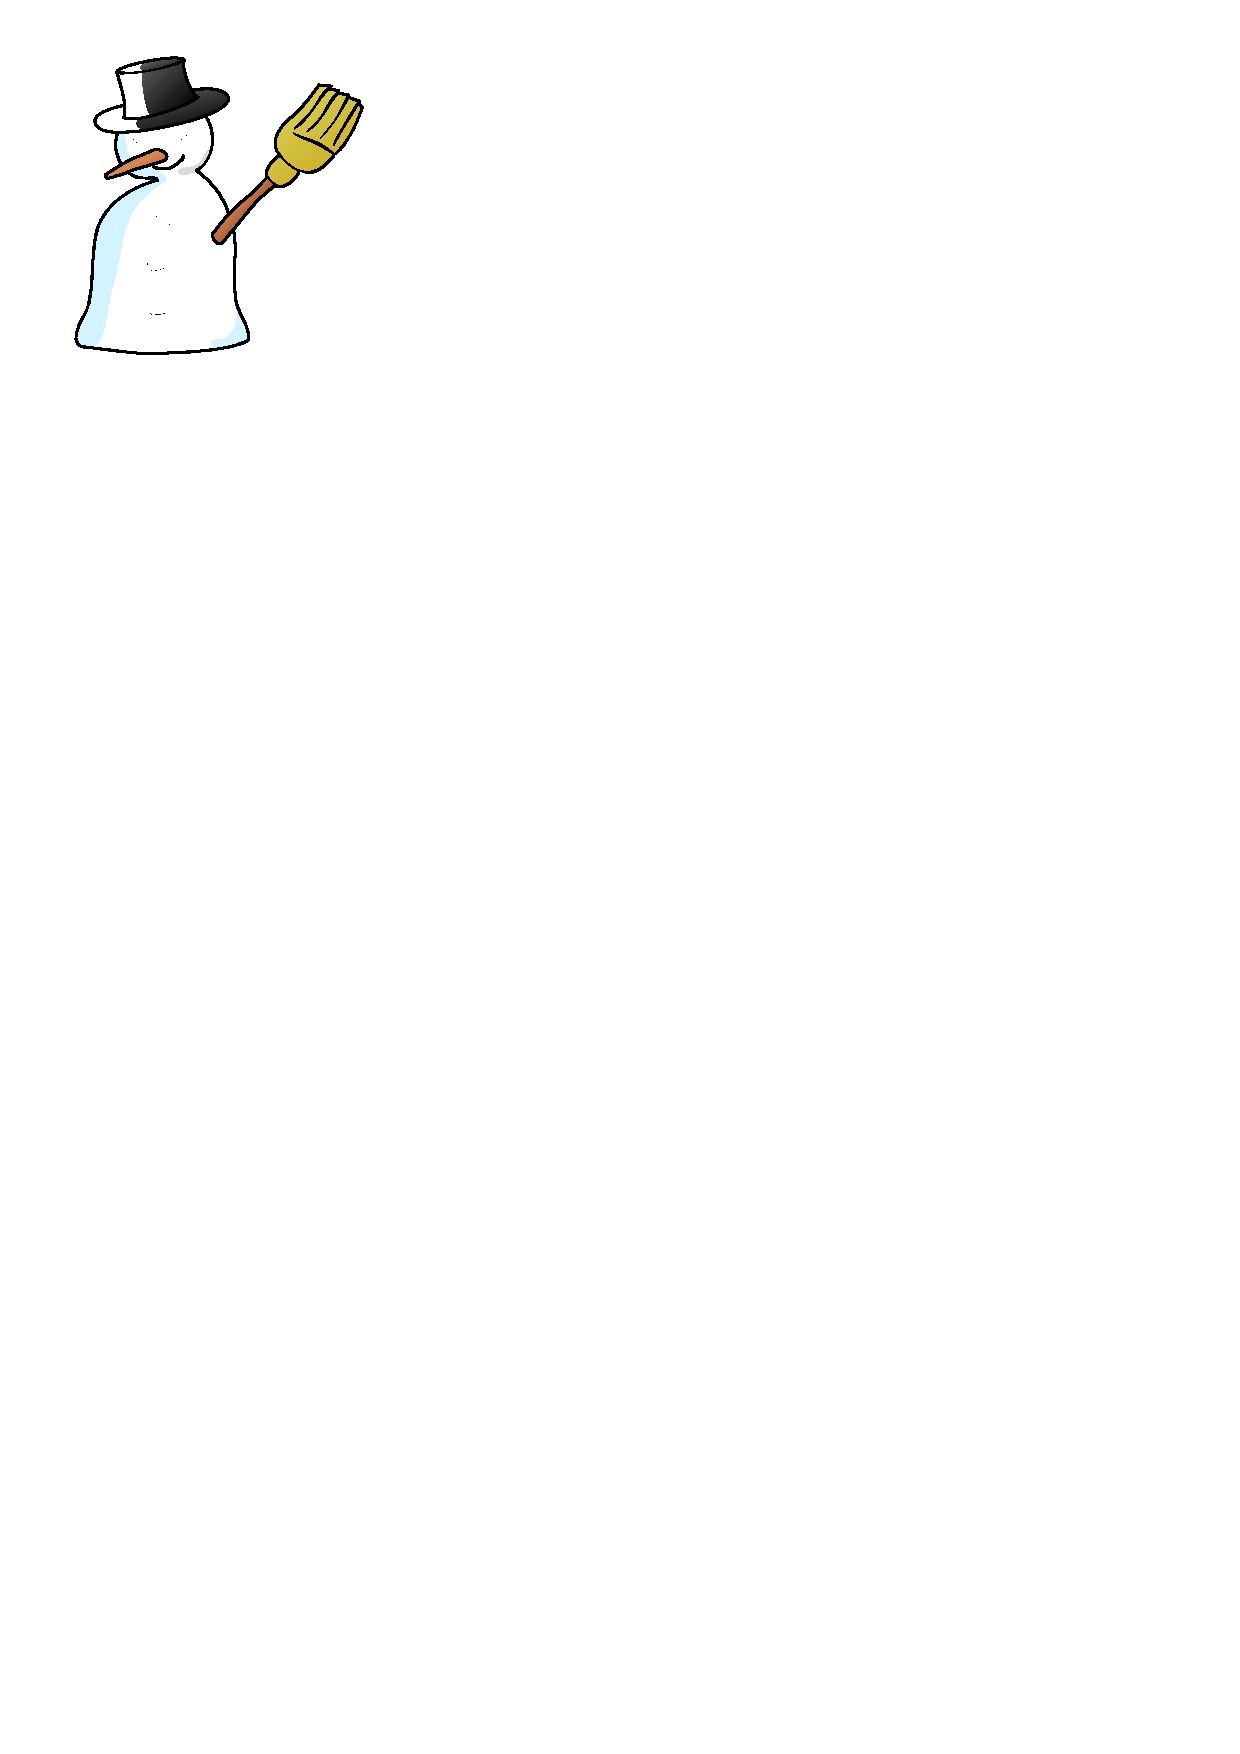
\includegraphics[width=2cm]{snowman-vectorial}
%   \caption{A snow-man}
% \end{wrapfigure}	
% 
% \noindent\verb!\usepackage{wrapfig}!\\
% This then gives you access to:\\
% \verb!\begin{wrapfigure}[lineheight]{alignment}{width}!\\
% Alignment can normally be either ``l'' for left, or ``r'' for right. Lowercase ``l'' or ``r'' forces the figure to start precisely where specified (and may cause it to run over page breaks), while capital ``L'' or ``R'' allows the figure to float. If you defined your document as twosided, the alignment can also be ``i'' for inside or ``o'' for outside, as well as ``I'' or ``O''. The width is obviously the width of the figure. The example above was introduced with:
% \lstset{language=TeX, morekeywords={\begin,\includegraphics,\caption}, caption=Wrapfig Example, label=lst:latex_example}
% \begin{lstlisting}
% 	\begin{wrapfigure}{l}{2.5cm}
% 	  \centering
% 	    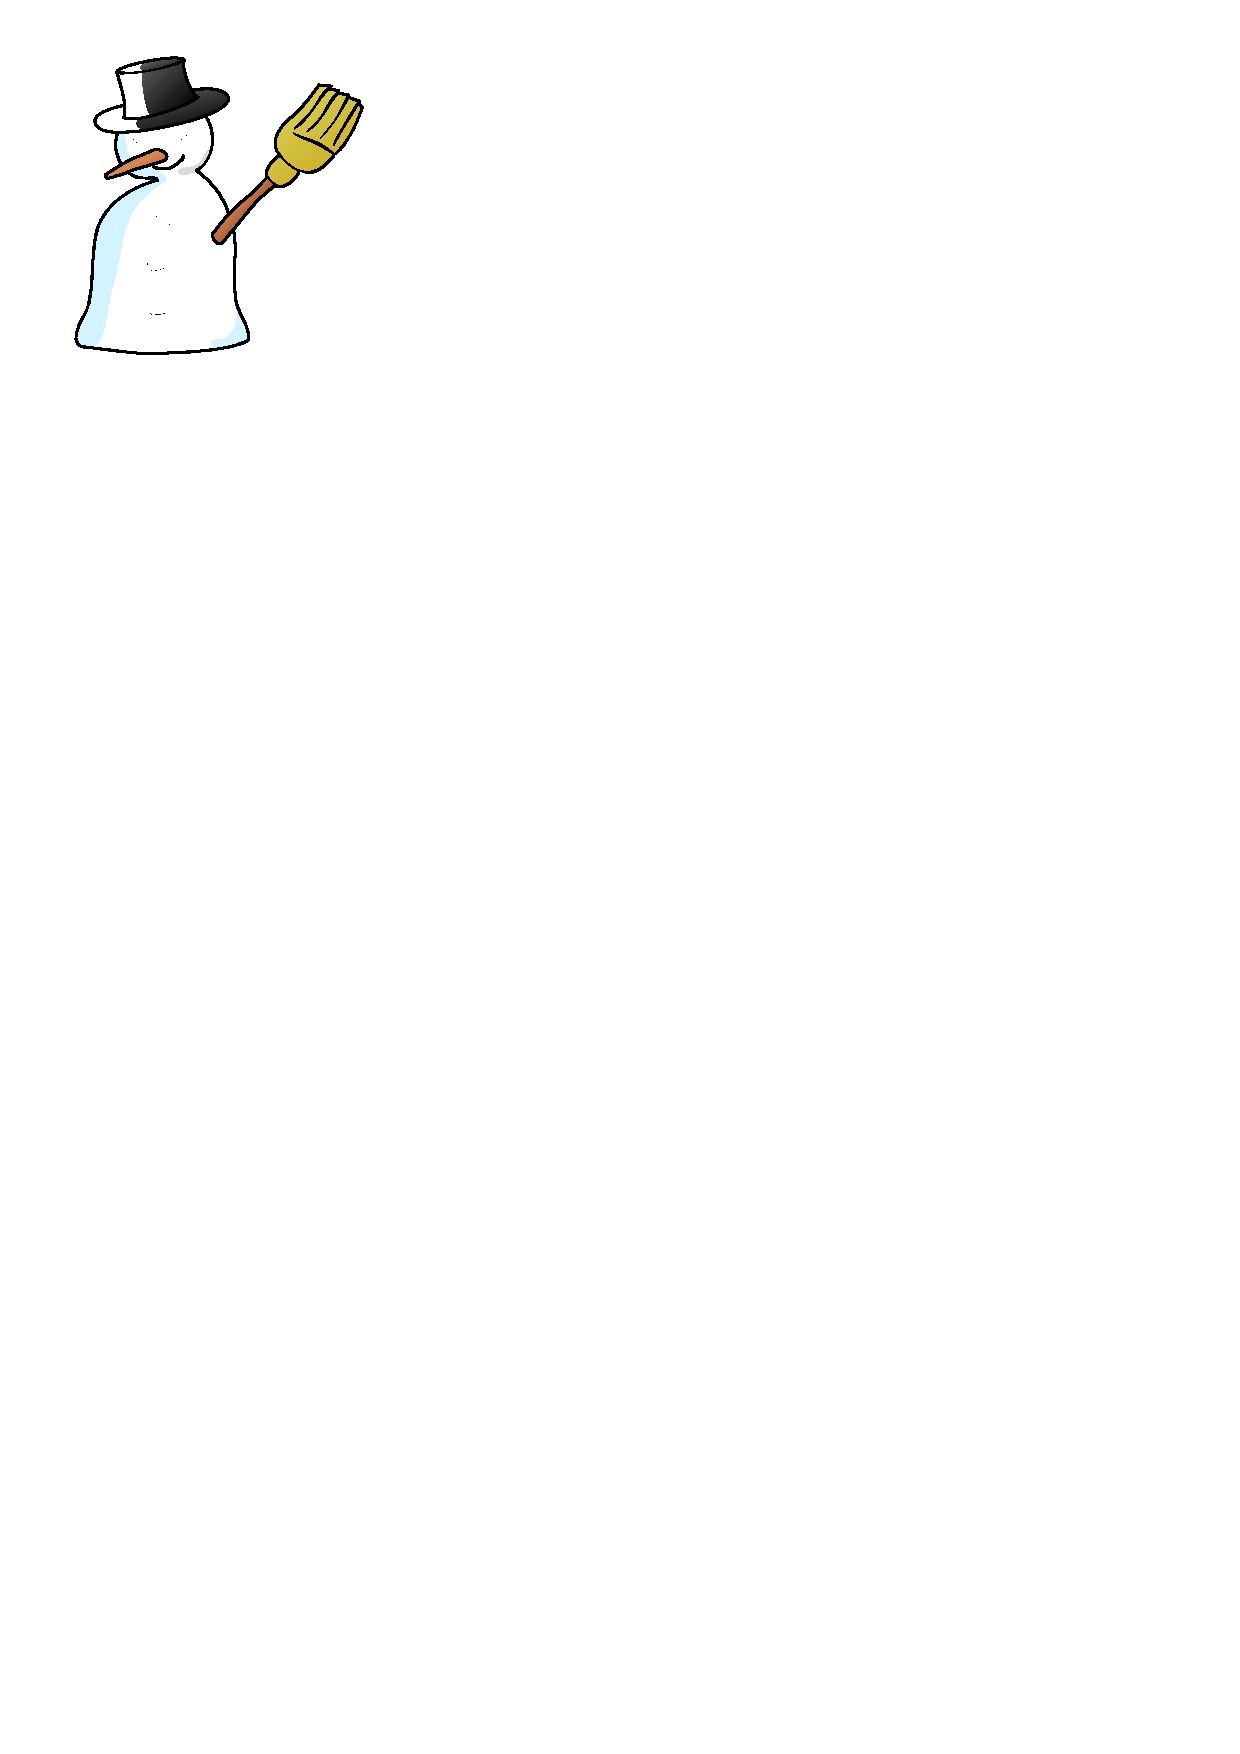
\includegraphics[width=2cm]{snowman-vectorial}
% 	  \caption{A snow-man}
% 	\end{wrapfigure}	
% \end{lstlisting}

% subsection inserting_images_wrapped_with_text (end)

% section floats_figures_and_captions (end)



%%%%%%%%%%%%%%%%%%%%%%%%%%%%%%%%%%%%%%%%%%%%%%%%%%%%%%%%%%%%%%%%%%%%
% Comments
\begin{comment}

\begin{figure}[htbp]
\centering
 \subbottom[One sub-figure]{%
    
\includegraphics[width=0.5\linewidth]{knitting-vectorial}}%
 \subbottom[Another sub-figure]{%
    
\includegraphics[width=0.5\linewidth]{knitting-vectorial}}
\caption{A figure with two sub-figures!}
\label{fig:fig2subfig}
\end{figure}






\newpage

{\Large To be included in the sections above}\\

Para fazer citações, deverá usar-se a chave da referência no ficheiro BibTeX. Se for uma única referência~\cite{Artho04}, usar um ``\verb!~!'' para ligar o \verb!\cite{...}! à palavra que o precede (\ldots\verb!referência~\cite{Artho04}!).  Caso queira fazer múltiplas citações~\cite{Shavit95,Silberschatz06,Moss85}, deverá agrupá-las dentro de um úinico \verb!\cite{...}!.

Note que o ficheiro de bibliografia pode ter tantas entradas quantas quiser. Apenas aquelas cuja chave seja referenciada no texto é que serão incluidas na listagem de bibliografia.


Footnotes\footnote{This is a simple footnote.} will be numbered and shown in the bottom of the page.


A Tabela~\ref{tab:hla:results} ilustra alguns conceitos importantes associados à contrução de tabelas:
\begin{asparaenum}[i)]
	\item Não usar linhas verticais;
	\item A legenda deve ficar por cima da tabela;
	\item Usar as macros \verb!\toprule!, \verb!\midrule! e \verb!\bottomrule! para fazer a linha horizontal superior, interiores e inferior, respectivamente.
\end{asparaenum}
 
\begin{table}[ht]
	\caption{Test results summary.}
	\label{tab:hla:results}
\centering
\begin{tabular}{lccccc}
	\toprule
	\multicolumn{1}{c}{\textbf{Test}} 	& \textbf{Anomalies}	& \textbf{Warnings}	& \textbf{Correct} 	& \textbf{Categories}		& \textbf{Missed} \\
	\midrule
\cite{Beckman08}~Connection 	& 2 & 2	& 1	& \emph{C}				& 1 \\
\cite{Artho03}~Coordinates'03 	& 1	& 4	& 1	& \emph{2B, 1C}			& 0 \\
\cite{Artho03}~Local Variable	& 1	& 2	& 1	& \emph{A}				& 0 \\
\cite{Artho03}~NASA				& 1	& 1	& 1	& ---					& 0 \\
\cite{Artho04}~Coordinates'04	& 1	& 4	& 1	& \emph{3C}				& 0 \\
\cite{Artho04}~Buffer			& 0	& 7	& 0	& \emph{2A, 1B, 2C, 2D}	& 0 \\
\cite{Artho04}~Double-Check		& 0	& 2	& 0	& \emph{1A, 1B}			& 0 \\
\cite{Flanagan04}~StringBuffer	& 1	& 0	& 0	& ---					& 1 \\
\cite{Praun03}~Account			& 1	& 1	& 1	& ---					& 0 \\
\cite{Praun03}~Jigsaw			& 1	& 2	& 1	& \emph{C}				& 0 \\
\cite{Praun03}~Over-reporting	& 0	& 2	& 0	& \emph{1A, 1C}			& 0 \\
\cite{Praun03}~Under-reporting	& 1	& 1	& 1	& ---					& 0 \\
\cite{IBM-Rep}~Allocate Vector	& 1	& 2	& 1	& \emph{C}				& 0 \\
Knight Moves					& 1	& 3	& 1	& \emph{2B}				& 0 \\
	\midrule
	\textbf{Total}			& \textbf{12}		& \textbf{33}		& \textbf{10}			& \textbf{5A, 6B, 10C, 2D}	& \textbf{2} \\
	\bottomrule
\end{tabular}
\end{table}



\begin{figure}[htbp]
	\centering
    \subbottom[Novelo de lã] {%
		\label{fig:novelo}
		
\includegraphics[height=1in]{knitting-vectorial}
    }
\qquad\qquad
    \subbottom[Tempestade com neve] {%
		\label{fig:nuvem}
		
\includegraphics[height=1in]{snowstorm-vectorial}
    }
  \caption{Exemplo de utilização de \emph{subbottom}}
  \label{fig:figura-completa}
\end{figure}


Para incluir listagens de código no seu documento, deverá incluir o pacote \emph{listings} e depois usar o ambiente \emph{lstlisting}, como exemplificado na Listagem~\ref{lst:HelloWorld}.

\lstset{language=Java, caption=Hello World, label=lst:HelloWorld}
\begin{lstlisting}
/** 
 * The HelloWorldApp class implements an application that
 * simply prints "Hello World!" to standard output.
 */
class HelloWorldApp {%
    public static void main(String[] args) {%
        System.out.println("Hello World!"); // Display the string.
    }
}
\end{lstlisting}


\end{comment}